\section{Related Work - Activity Forecasting}

\begin{frame}
	\frametitle{}
	
	\Huge
	
	\vspace{0.5cm}
	
	\begin{center}
		\textbf{Inverse Reinforcement Learning}
	\end{center}
\end{frame}

\begin{frame}
	\frametitle{Reinforcement Learning}
	
	\begin{center}
		\begin{tikzpicture}
			\node at (0,0) [draw=white,ultra thick,inner sep=0pt]
			{
				\includegraphics[scale=0.2]{Figures/RL}
			};
		\end{tikzpicture}
	\end{center}
	
	\vspace{-0.5cm}
	
	\textcolor{red}{Inverse RL:} \\
	\hspace{1cm}\textcolor{red}{Given $ \pi^* $ and $ T $, can we recover $ R $?\\
	\hspace{1cm}More generally, given execution traces, can we recover $ R $?}
\end{frame}

\begin{frame}
	\frametitle{Motivation for Inverse RL}
	
	\Large
	
	\vspace{0.3cm}
	
	\begin{itemize}
		\item \textbf{Scientific inquiry}
			  \begin{itemize}
				  \item Model animal and human behaviour (\emph{Russell et al.}, 2000)
				  \vspace{0.15cm}
				  \item Activity forecasting (\emph{Ziebart et al.}, 2012)
			  \end{itemize}
		\vspace{0.2cm}
		\item \textbf{Imitation learning}
			  \begin{itemize}
				  \item Presupposition: reward function provides the most succinct and
				  		transferable definition of the task
				  \vspace{0.15cm}
				  \item Has enabled advancing the state-of-the-art in various robotic domains
			  \end{itemize}
		\vspace{0.2cm}
		\item \textbf{Agent modelling (adversarial and cooperative)}
		\vspace{0.2cm}
		\item ...
	\end{itemize}
\end{frame}

\begin{frame}
	\frametitle{Theoretical Concepts}
	\framesubtitle{Markov Decision Process}
	
	\Large
	
	\vspace{0.3cm}
	
	A (finite) discrete-time MDP is a tuple $ (\mathbf{S},\mathbf{A},\mathbf{P}_{sa},
	\mathbf{R},\gamma) $:
	\vspace{0.1cm}
	\begin{itemize}
		\item $ \mathbf{S} $ is a finite set of $ N $ states
		\vspace{0.1cm}
		\item $ \mathbf{A} = \{ a_1, a_2, \ldots, a_k \} $ is a set of $ k $ actions
		\vspace{0.1cm}
		\item $ \mathbf{P}_{sa}(\cdot) $ are the state transition probabilities upon taking
			  action $ a $ in a state $ s $
		\vspace{0.1cm}
		\item $ \mathbf{R} : \mathbf{S} \times \mathbf{A}  \mapsto \mathds{R} $ is the
			  reinforcement function, bounded in absolute value by $ R_{max} $
		\vspace{0.1cm}
		\item $ \gamma \in [0,1) $ is the discount factor
		\vspace{0.1cm}
	\end{itemize}
\end{frame}

\begin{frame}
	\frametitle{Theoretical Concepts}
	\framesubtitle{Value Function}
	
	\Large
	
	\vspace{0.2cm}
	
	A \textbf{policy} is defined as any map $ \pi : \mathbf{S} \mapsto \mathbf{A} $ and the
	\textbf{value function} for a policy $ \pi $, evaluated at any state $ s_1 $ is given by\\
	
	\vspace{-0.5cm}
	
	\begin{equation*}
		V^\pi(s_1) = E \, \Big [ \, R(s_1) + \gamma R(s_2) + \gamma^2 R(s_3) + \cdots \; | \;
		\pi \, \Big ]
	\end{equation*}
	
	where the expectation is over the distribution of the state sequence ($ s_1, s_2, \ldots,
	s_N $) we pass through, when we execute the policy $ \pi $ starting from $ s_1 $\\
\end{frame}

\begin{frame}
	\frametitle{Theoretical Concepts}
	\framesubtitle{Q-function}
	
	\Large
	
	The \textbf{Q-function} is defined as
	
	\begin{equation*}
		Q^\pi(s,a) = \mathbf{R}(s) + \gamma E_{s^\prime \sim \mathbf{P}_{sa}(\cdot)} \big [
		V^\pi(s^\prime) \big ]
	\end{equation*}
	
	\vspace{0.5cm}
	
	where the notation $ s^\prime \sim \mathbf{P}_{sa}(\cdot) $ means the expectation is with
	respect to $ s^\prime $ distributed according to $ \mathbf{P}_{sa}(\cdot) $.\\
\end{frame}

\begin{frame}
	\frametitle{Theoretical Concepts}
	\framesubtitle{Bellman Equations}
	
	\Large
	
	\vspace{0.3cm}
	
	Let a MDP $ \mathcal{M} = (\mathbf{S},\mathbf{A},\mathbf{P}_{sa},\mathbf{R},\gamma) $ and a
	policy $ \pi : \mathbf{S} \mapsto \mathbf{A} $ be given. Then, for all $ s \in \mathbf{S} $,
	$ a \in \mathbf{A} $, $ V^\pi $ and $ Q^\pi $ satisfy
	
	\vspace{-0.2cm}
	
	\begin{eqnarray*}
		V^\pi(s) &=& \mathbf{R}(s) + \gamma \sum_{s^\prime} \mathbf{P}_{s\pi(s)}(s^\prime)V^\pi(s^\prime)\\
		Q^\pi(s,a) &=& \mathbf{R}(s) + \gamma \sum_{s^\prime} \mathbf{P}_{sa}(s^\prime)V^\pi(s^\prime)
	\end{eqnarray*}
\end{frame}

\begin{frame}
	\frametitle{Theoretical Concepts}
	\framesubtitle{Bellman Optimality}
	
	\Large
	
	Let a MDP $ \mathcal{M} = (\mathbf{S},\mathbf{A},\mathbf{P}_{sa},\mathbf{R},\gamma) $ and a
	policy $ \pi : \mathbf{S} \mapsto \mathbf{A} $ be given. Then $ \pi $ is an \textbf{optimal
	policy} for $ \mathcal{M} $ if and only if, for all $ s \in \mathbf{S} $\\
	
	\begin{equation*}
		\pi(s) \in \arg \max_{a \, \in \, \mathbf{A}} Q^\pi(s,a)
	\end{equation*}
\end{frame}

\begin{frame}
	\frametitle{Theoretical Concepts}
	\framesubtitle{Policy Optimality}
	
	\Large
	
	Let a finite state space $ \mathbf{S} $, a set of transition probabilities matrices $ \{
	\mathbf{P}_{a} \} $, a set of actions $ \mathbf{A} = \{a_1,\ldots,a_k\} $ and a discount
	factor $ \gamma \in [0,1) $ be given. Then, the policy $ \pi $, given by $ \pi(s) \equiv a_*
	$, is \textbf{optimal} if and only if, for all $ a \in \mathbf{A} $, the reward $ \mathbf{R}
	$ satisfies\\
	
	\begin{equation*}
		(\mathbf{P}_{a_*} - \mathbf{P}_a)(\mathbf{I} - \gamma \mathbf{P}_{a_*})^{-1} \,
		\mathbf{R} \succeq 0
	\end{equation*}
\end{frame}

\begin{frame}
	\frametitle{IRL Problem Definition}
	
	\Large
	
	\begin{equation*}
		\begin{array}{ll}
			\max \sum\limits_{i=1}^N \min\limits_{a \in \mathbf{A}} \Big
			\{ \big [ \mathbf{P}_{a_*}(i) - \mathbf{P}_a(i) \big ] ( \mathbf{I} - \gamma
			\mathbf{P}_{a_*})^{-1} \mathbf{R} \Big \} - \lambda \| \mathbf{R} \|_1 \\ \\
			s.t. \\ \;\;\;\;
			\left \{
				\begin{array}{ll}
					(\mathbf{P}_{a_*} - \mathbf{P}_a)(\mathbf{I} - \gamma
					\mathbf{P}_{a_*})^{-1} \, \mathbf{R} \succeq 0 \;\,\,\,\, \forall \, a \in
					\mathbf{A} \\ \\
					| \mathbf{R}_i | \leq R_{max} \;\;\;\;\;\;\;\;\;\;\;\;\;\;\;\;\;\;\;\;\;\
					\;\;\;\;\;\;\;\;\,\,\,\,\, i \, \in \{ 1, \ldots, N \}
				\end{array}
			\right.
			\vspace{0.2cm}
		\end{array}
	\end{equation*}
\end{frame}

\begin{frame}
	\frametitle{Toward a Linear Program Definition}
	
	\Large
	
	\vspace{0.4cm}
	
	The \emph{non-linear} 1-norm operator $ \| \mathbf{R} \|_1 $ of the original problem should
	be linearized by adding two more variables $ r_i^+ $ and $ r_i^- $ for every $ r_i $
	variable with $ i \, \in \{ 1, \ldots, N \} $.
	
	\vspace{0.8cm}
	
	The \emph{non-linear} operator $ \min\limits_{a \in \mathbf{A}} $, instead, should be
	linearized by introducing $ N $ new variables $ x_i $ where $ i \, \in \{ 1, \ldots, N \} $
\end{frame}

\begin{frame}
	\frametitle{IRL Linear Program Definition}
	
	\Large
	
	\vspace{-0.3cm}
	
	\begin{equation*}
		\begin{array}{ll}
			\min \sum\limits_{i=1}^N -x_i + \lambda (r_i^+ - r_i^-)
			\vspace{-0.35cm} \\ \\
			s.t. \\ \;\;\;\;
			\left \{
				\begin{array}{ll}
					x_i \leq (\mathbf{P}_{a_*} - \mathbf{P}_a)(\mathbf{I} - \gamma
					\mathbf{P}_{a_*})^{-1} \mathbf{R} \\
					\vspace{-0.25cm} \\
					\;\;\;\;\;\;\;\;\;\,\,\;\;\;\;\;\;\;\;\;\;\;\;\;\;\;\;\;\;\;\;\;\;\;\;\;\;
					\;\;\; \forall \, a \in \mathbf{A}, \; i \in \{ 1, \ldots, N \}
					\vspace{-0.25cm}\\ \\
					x_i \geq 0 \;\;\;\;\;\;\,\,\,\,\;\;\;\,\,\,\,\,\;\,\,\,\,\,\,\,\;\;\;\;\;
					\;\;\;\;\;\;\;\;\;\;\;\;\;\,\,\;\,\,\,\,\,\, i \, \in \{ 1, \ldots, N \}
					\vspace{-0.25cm} \\ \\
					r_i = r_i^+ + r_i^- \;\,\,\,\,\,\;\,\,\,\,\,\,\,\;\;\;\;\;
					\;\;\;\;\;\;\;\;\;\;\;\;\,\,\,\,\,\,\,\,\,\,\,\,\, i \, \in \{ 1, \ldots, N \}
					\vspace{-0.25cm}
					\\ \\
					| \mathbf{R}_i | \leq R_{max} \;\;\;\;\;\;\;\;\;\;\;\,\,\,\,\;\;\
					\;\;\;\;\;\;\;\;\;\;\;\,\,\;\;\;\,\,\,\,\,\, i \, \in \{ 1, \ldots, N \}
				\end{array}
			\right.
			\vspace{0.2cm}
		\end{array}
	\end{equation*}
\end{frame}

\begin{frame}
	\frametitle{A Simple Example}
	
	\vspace{0.1cm}
	
	\begin{center}
		\begin{tikzpicture}
			\node at (0,0) [draw=white,ultra thick,inner sep=0pt]
			{
				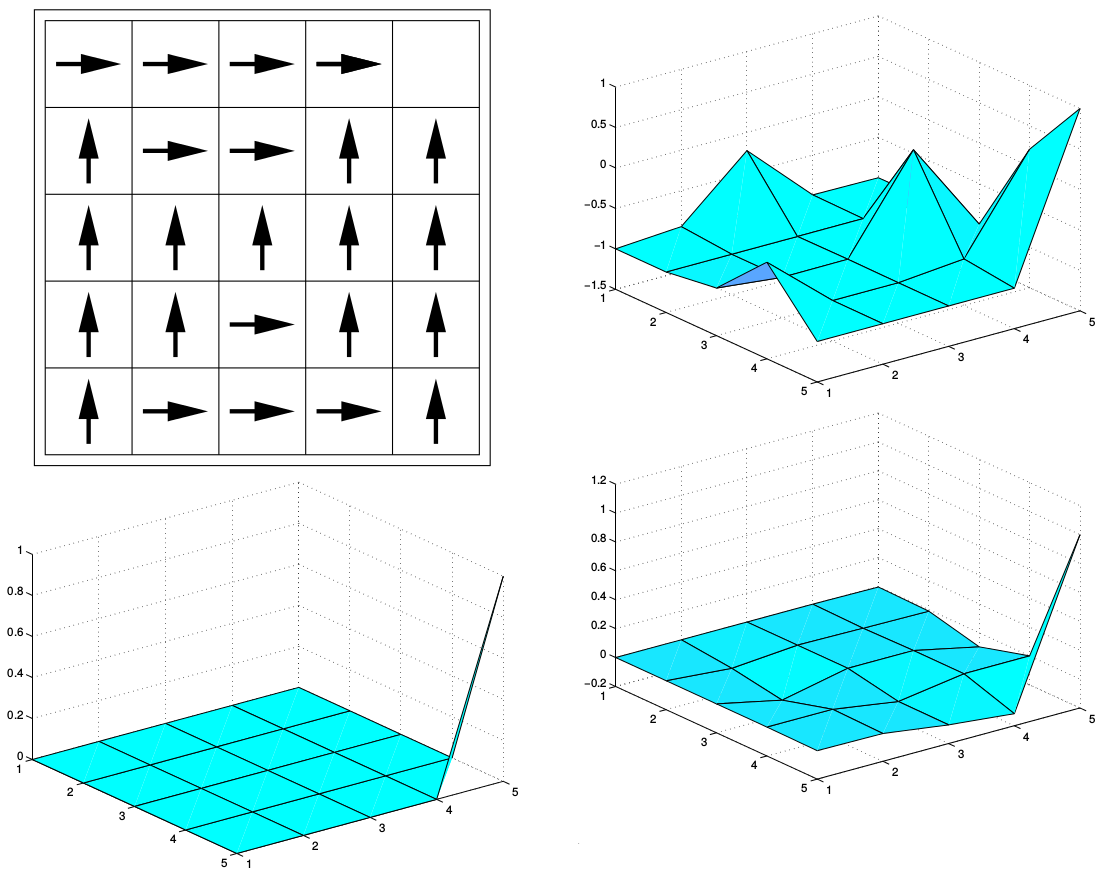
\includegraphics[scale=0.23]{Figures/GridExample}
			};
		\end{tikzpicture}
	\end{center}
\end{frame}

\begin{frame}
	\frametitle{}
	
	\Huge
	
	\vspace{0.5cm}
	
	\begin{center}
		\textbf{Activity Forecasting}
	\end{center}
\end{frame}

\begin{frame}
	\frametitle{Related Work}
	\framesubtitle{Human Activity Classification and Activity Recognition}
	
	\vspace{0.4cm}
	
	\begin{columns}[T]
		\column{.55\textwidth}
		
		\vspace{0.2cm}
		
		\begin{itemize}
			\item \textbf{Nascimento {et al.} \cite{Nascimento10}:} recognise pedestrian trajectories in
				  video sequences, in a surveillance context
			
			\vspace{1.2cm}
			
			\item \textbf{Veloso {et al.} \cite{Vail07}:} discriminatively trained Conditional Random
				  Fields for activity recognition
		\end{itemize}
		
		\column{.5\textwidth}
		
		\centering
		\begin{tikzpicture}
			\node at (1.42,0) [draw=black,ultra thick,inner sep=0pt]
			{
				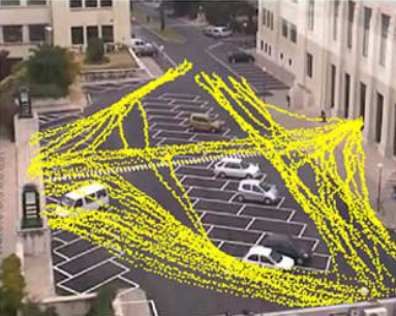
\includegraphics[height=2.2cm]{Figures/Nascimento-1}
			};
			\node at (-1.42,0) [draw=black,ultra thick,inner sep=0pt]
			{
				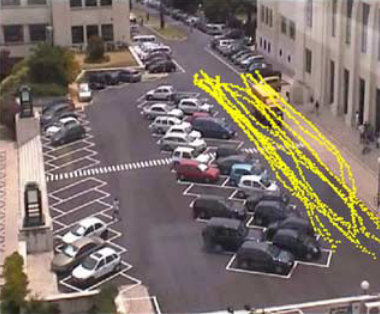
\includegraphics[height=2.2cm]{Figures/Nascimento-2}
			};
			\node at (0,-2.8) [draw=black,ultra thick,inner sep=0pt]
			{
				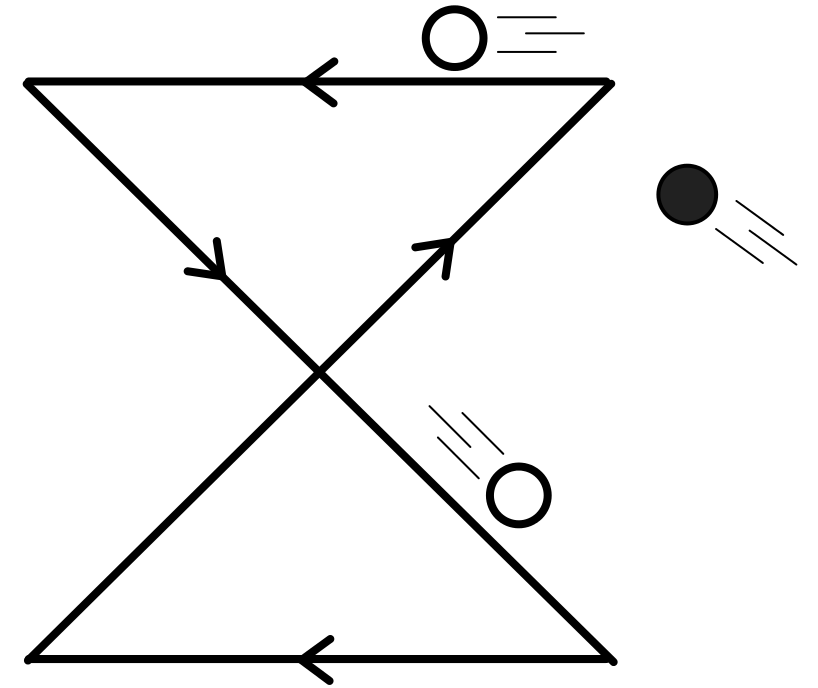
\includegraphics[width=3.6cm]{Figures/Veloso}
			};
		\end{tikzpicture}
	\end{columns}
	
	\vspace{0.47cm}
	
	\tiny
	
	\cite{Nascimento10} J. C. Nascimento \emph{et al.}, ``Trajectory classification using switched
	dynamical hidden Markov models'', Image Processing, 2010
	
	\vspace{-0.17cm}
	
	\cite{Vail07} D. L. Vail \emph{et al.}, ``Conditional random fields for activity recognition'',
	AAMAS, 2007
\end{frame}

\begin{frame}
	\frametitle{Related Work}
	\framesubtitle{Activity Forecasting through Semantic Mapping}
	
	\vspace{0.33cm}
	
	\large
	
	\textbf{Ziebart \emph{et al.} \cite{Kitani12}} propose a method for activity forecasting by
	combining:
	
	\begin{itemize}
		\item Semantic scene understanding
		\vspace{0.05cm}
		\item Inverse Optimal Control
	\end{itemize}
	
	\vspace{-0.2cm}
	
	\begin{center}
		\begin{tikzpicture}
			\node at (0,0) [draw=white,ultra thick,inner sep=0pt]
			{
				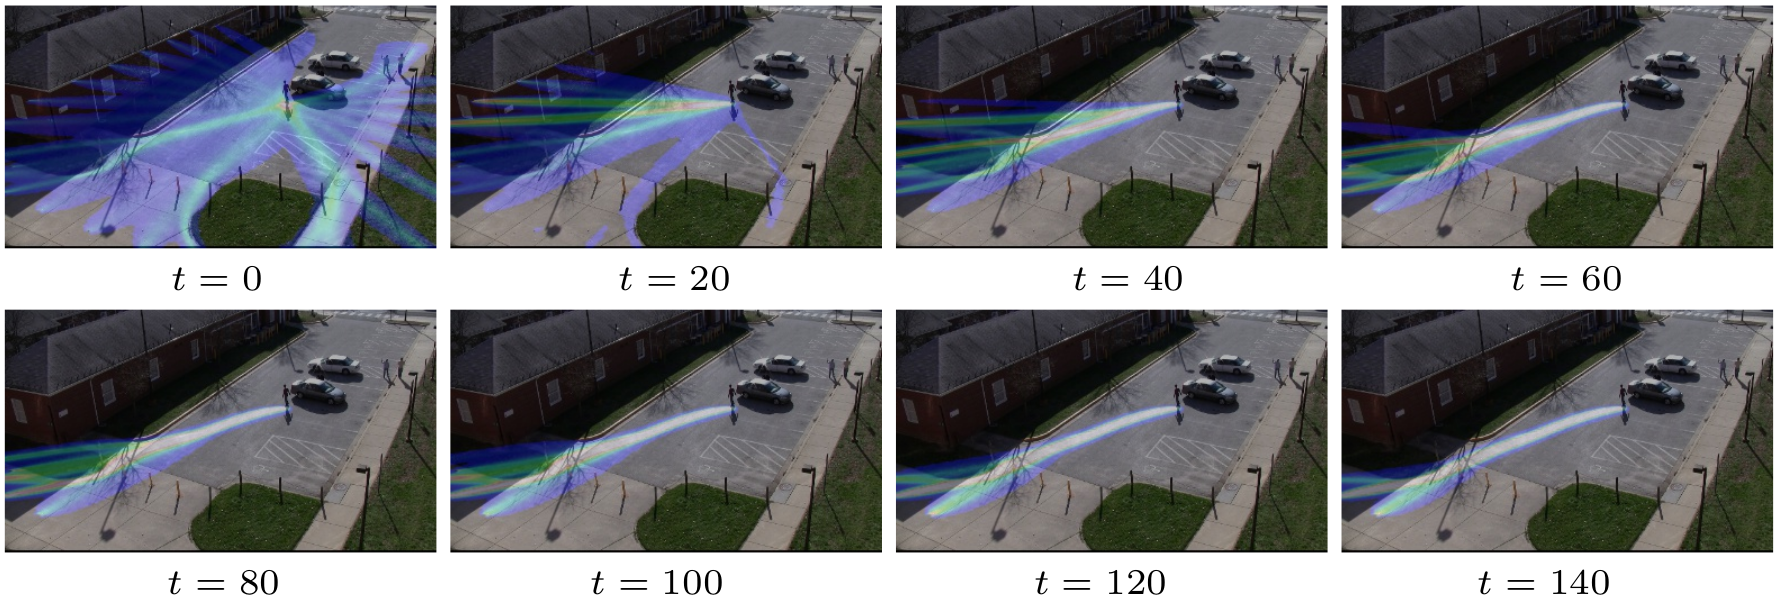
\includegraphics[scale=0.19]{Figures/ActivityForecasting}
			};
		\end{tikzpicture}
	\end{center}
	
	\vspace{-0.3cm}
	
	\tiny
	
	\cite{Kitani12} K. Kitani \emph{et al.}, ``Activity Forecasting'', ECCV, 2012
\end{frame}

\begin{frame}
	\frametitle{Advantages/Disadvantages}
	
	\Large
	
	\vspace{0.4cm}
	
	\underline{\textbf{Advantages}} \\
	
	\vspace{0.2cm}
	
	\begin{itemize}
		\item Knowledge transfer by using physical scene features
		\item Accurate and robust destination forecasting
	\end{itemize}
	
	\vspace{0.2cm}
	
	\underline{\textbf{Disadvantages}} \\
	
	\vspace{0.19cm}
	
	\begin{itemize}
		\item Prior knowledge of potential goals
		\item Space of possible motions is explicitly parametrised
		\item Applicability in dynamic environments? \\
			  \vspace{-0.2cm}
			  \begin{tabbing}
				  \hspace{0.3cm}
				  \large
				  $ \leadsto $ \emph{rescue or rapidly changing construction environment}
			  \end{tabbing}
	\end{itemize}
\end{frame}
